\documentclass[aspectratio=169]{beamer}
\usepackage[utf8]{inputenc}
\usepackage{utopia} %font utopia imported
\usetheme{Madrid}
\usecolortheme{default}

\usepackage{pgfplots}
\usepackage{tikz}
\usepackage[european resistor, european voltage, european current]{circuitikz}
\usetikzlibrary{arrows,shapes,positioning}
\usetikzlibrary{decorations.markings,decorations.pathmorphing,
decorations.pathreplacing}
\usetikzlibrary{calc,patterns,shapes.geometric}

%Information to be included in the title page:
\title{Cours d'introduction à la chimie quantique}

\subtitle{Chapitre 3 : Système simple\\Partie 2 :Oscillateur harmonique}
\author{François Dion}
%\institute{Overleaf}
\date{2020}




%\logo{\includegraphics[height=1.5cm]{lion-logo.jpg}}

%End of title page configuration block
%------------------------------------------------------------



%------------------------------------------------------------
%The next block of commands puts the table of contents at the 
%beginning of each section and highlights the current section:

%\AtBeginSection[]
%{
  %\begin{frame}
    %\frametitle{Table of Contents}
    %\tableofcontents[currentsection]
  %\end{frame}
%}
%------------------------------------------------------------


\begin{document}

%The next statement creates the title page.
\frame{\titlepage}


%---------------------------------------------------------
%This block of code is for the table of contents after
%the title page
%\begin{frame}
%\frametitle{Table of Contents}
%\tableofcontents
%\end{frame}
%---------------------------------------------------------


\section{Le potentiel}
\begin{frame}
\frametitle{Le potentiel}
\begin{columns}
\column{0.5\textwidth}
Le potentiel considéré est le cas où:
%|x| = \begin{cases} x &\text{if }x \ge 0 \\ -x &\text{if }x < 0 \end{cases}
%\begin{equation}
%\begin{eqnarray}
%\begin{eqnarray*}
%V(x) &=& 


\begin{equation} \tag{1}
V(x)=kx^2
\end{equation} 
\column{0.5\textwidth}
\begin{figure}
\includegraphics[scale=0.4]{Pot}
\caption{Shéma représentant le potentiel d'un oscillateur harmonique}
\end{figure}


\end{columns}
\end{frame}


\begin{frame}

\begin{figure}
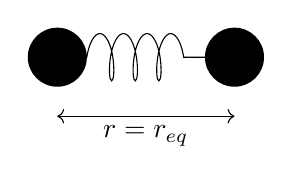
\begin{tikzpicture} [scale=0.75, decoration={coil,aspect=0.4,segment length=3mm,amplitude=3mm}]
%decoration : gère l'aspect du ressort par l'instruction decorate
\tikzset{ressort/.style={thick,gray,length=3mm}} %définition d'un style de ressort
\fill (150,0) circle (0.5);
%\draw[latex'-latex',double] (150,-5) -- node[label=r_eq] {} (153,-5);
%\draw[latex'-latex',double] (150,-1.0) -- node[] {$r=r_{eq}$} (153,-1.0);
\draw[decoration={aspect=0.3, segment length=3.0mm, amplitude=3mm,coil},decorate,rotate=0] (150.5,0)--(152.5,0) node [right=0cm,black] {};
\path[<->] (150,-1.0) edge node[below] {$r=r_{eq}$} (153,-1.0);

\fill (153.0,0) circle (0.5);
\end{tikzpicture}

\includegraphics[scale=0.5]{Pot_req}
\caption{Shéma représentant le potentiel d'un oscillateur harmonique}
\end{figure}
\end{frame}
%
%%https://fr.wikipedia.org/wiki/Oscillateur_harmonique_quantique#/media/Fichier:Morse-potential-fr.png


\begin{frame}

\begin{figure}
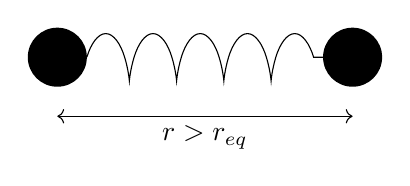
\begin{tikzpicture} [scale=0.75, decoration={coil,aspect=0.4,segment length=3mm,amplitude=3mm}]
%decoration : gère l'aspect du ressort par l'instruction decorate
\tikzset{ressort/.style={thick,gray,smooth}} %définition d'un style de ressort
\fill (149,0) circle (0.5);
\draw[decoration={aspect=0.3, segment length=6.0mm, amplitude=3mm,coil},decorate,rotate=0] (149.5,0)--(153.5,0) node [right=0cm,black] {};
\path[<->] (149,-1.0) edge node[below] {$r>r_{eq}$} (154,-1.0);
\fill (154.0,0) circle (0.5);
\end{tikzpicture}

\includegraphics[scale=0.5]{Pot_r_1}
\caption{Shéma représentant le potentiel d'un oscillateur harmonique}
\end{figure}
\end{frame}

\begin{frame}

\begin{figure}
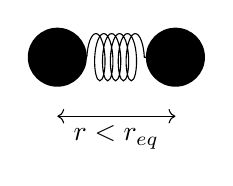
\begin{tikzpicture} [scale=0.75, decoration={coil,aspect=0.4,segment length=3mm,amplitude=3mm}]
%decoration : gère l'aspect du ressort par l'instruction decorate
\tikzset{ressort/.style={thick,gray,smooth}} %définition d'un style de ressort
\fill (150.5,0) circle (0.5);
\draw[decoration={aspect=0.3, segment length=1.0mm, amplitude=3mm,coil},decorate,rotate=0] (151.0,0)--(152.0,0) node [right=0cm,black] {};
\path[<->] (150.5,-1.0) edge node[below] {$r<r_{eq}$} (152.5,-1.0);
\fill (152.5,0) circle (0.5);
\end{tikzpicture}

\includegraphics[scale=0.5]{Pot_r_m1}
\caption{Shéma représentant le potentiel d'un oscillateur harmonique}
\end{figure}
\end{frame}


\section{L'Hamiltonien}
\begin{frame}
\frametitle{Le potentiel}

L'Hamiltonien général d'un système conservatif unidimensionnel est

\begin{equation}\tag{2}
\hat{H}=-\frac{\hbar^2}{2m}\frac{\partial^2}{\partial x^2}+\hat{V}(x)
\end{equation} 


\end{frame}


\begin{frame}
\frametitle{l'Hamiltonien}

L'Hamiltonien de ce système est

\begin{equation}\tag{2}
\hat{H}=-\frac{\hbar^2}{2m}\frac{\partial^2}{\partial x^2}+k\hat{x}^2
\end{equation} 



\end{frame}

\section{L'Hamiltonien}
\begin{frame}
\frametitle{Équations de Shrodinger indépendante du temps}
Rappelons l'équation de Shrodinger indépendante du temps
\begin{equation}
\hat{H}\Psi(x)=E\Psi(x)
\end{equation}
Les solutions sont de la forme
\begin{equation}
\Psi_{\nu}(x)=N_{\nu}H_{\nu}(y)e^{\frac{-y^2}{2}}
\end{equation}
o\'u $N_{\nu}$ est une constante de normalisation, $H_{\nu}(y)$ est un polynome d'Hermite et $y=\frac{x}{\alpha}, \alpha=(\frac{\hbar^2}{mk})^{\frac{1}{4}}$

\end{frame}

\begin{frame}
\frametitle{Équations de Shrodinger indépendante du temps}
Les premiers polynomes d'Hermite sont 
\begin{table}
\begin{tabular}{ c | c }
n & $H(x)$ \\\hline
0 & $1$  \\
1 & $2x$ \\
2 & $4x^2-2$ \\
3 & $8x^3-12x$ \\
4 & $16x^4-48x^2+12$  \\
\end{tabular} 
\end{table}

\end{frame}

%
\section{L'Hamiltonien}
\begin{frame}
\frametitle{Équations de Shrodinger indépendante du temps}
L'énegie de ces états est
\begin{equation}
E_{\nu}=\left(\nu+\frac{1}{2}\right)\hbar\nu
\end{equation}

La différence d'énegie entre les états est constantes
\begin{equation}
E_{\nu+1}-E_{\nu}=\hbar \omega
\end{equation}
\end{frame}



\begin{frame}
\frametitle{Le potentiel}
\begin{figure}
\includegraphics[scale=0.6]{fct_propre}
\caption{Shéma représentant le potentiel d'un oscillateur harmonique}
\end{figure}
\end{frame}

\begin{frame}
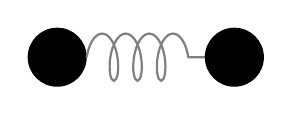
\begin{tikzpicture} [scale=0.75, decoration={coil,aspect=0.4,segment length=3mm,amplitude=3mm}]
%decoration : gère l'aspect du ressort par l'instruction decorate
\tikzset{ressort/.style={thick,gray,smooth}} %définition d'un style de ressort



\fill (0,0) circle (0.5);
\draw[ressort,decorate,rotate=0] (0.5,0)--(2.5,0) node [right=0cm,black] {};
\fill (3.0,0) circle (0.5);
\end{tikzpicture}

\end{frame}
\end{document}



